
%%%%%%%%%%%%%%%%%%%%%%%%%%%%%%%%%%%%%%%%%%%%%%%%%%%%%%%%%%%%%%%%%%%%%%%%%
%           Capítulo 2: MARCO TEÓRICO - REVISIÓN DE LITERATURA
%%%%%%%%%%%%%%%%%%%%%%%%%%%%%%%%%%%%%%%%%%%%%%%%%%%%%%%%%%%%%%%%%%%%%%%%%

\chapter{Marco teórico}

\section{Calculo de capacidad de corriente en pistas de circuitos impresos}



Antes de comenzar con la fabricación de un diseño de PCBs se debe de considerar el tamaño de pistas necesarios para el manejo de corrientes para cada circuito desarrollado, por esa razón mediante un análisis se debe avanzar en el diseño.\\

En la actualidad los requerimientos de corriente llevan a reducir el ancho de las pistas y espacios debido a que se desarrollan componentes cada vez más pequeños y sistemas igualmente más compactos, esto obliga al desarrollador a adaptarse a estos nuevos requerimientos.\\

Para encontrar una solución a esta eventualidad es necesario recurrir a estudios en estos temas que nos permita acercarnos al límite y para ello debemos de considerar todos los parámetros que influyan en nuestro sistema, obteniendo así resultados más precisos. En nuestro caso nos basaremos en los gráficos publicados en el IPC2152 \cite{IPC 2152} ``Standard for Determining Current Carry Capacity in Printed Board Design'' en 2009, este estándar es ampliamente utilizado en muchos proyectos que requieran este tipo de análisis. \\

Para el correcto entendimiento de los procesos que influyen en las pistas por el paso de la corriente debemos de recordar que el paso de la corriente por un conductor produce en este una caída de potencial que esta gobernada por la ley de OHM (R=V/I), esta caída de potencial se disipa en forma de calor por el efecto Joule $Q=I^{2}Rt$. En nuestro el conductor es nuestra pista, su resistencia depende de varios factores, pero lo principal es su sección (ancho x espesor) y su longitud. El efecto térmico es en realidad el que nos interesa conocer al momento del dimensionamiento de la PCB. Por esta razón, para poder calcular una capacidad de transporte de corriente, hay que analizarlo en términos de incremento de temperatura. Fijando como un incremento maxico admisible.\\

Existen algunos parámetros que se deben de considerar importantes de conocer, ya que los mismos alteran o modifican el comportamiento termico de la pista, afectando de manera significativa, los mas importantes son:\\

\begin{itemize}
\item Corriente eléctrica que circula.
\item Tipo de material base.
\item Calculo de corriente de pistas.
\item Sección de la pista.
\item Espesor del laminado de cobre.
\item Espesor de la placa.
\item Presencia de planos de tierra o grandes áreas de cobre.
\item Ambiente de aplicación (gabinete, forzadores de aire, vacío, etc.)
\end{itemize}

Considerar todos estos parámetros en un modelo es bastante complicado, tanto que, en sí, el estándar fue fijado por medio de ensayos y presentando los resultados en forma de curvas. Mediante estos datos empíricos se hace una aproximación que se acerque al límite que deseamos, tomando en cuenta que es importante sobredimensionar dichos límites. \\

El cálculo que se realiza se basa en el fijado de una variación máxima de temperaturas admisibles. La variación térmica se define como un aumento de temperatura por encima de la temperatura inicial que experimenta el conductor. \\
Para el cálculo se requieren los gráficos ya antes mencionados que son dos. El primer grafico es una de las tres entradas y se trata de una serie de curvas que corresponden a los incrementos de temperatura desde diez a cien grados centígrados. En el eje de las ordenadas se grafica la corriente máxima en amperes y en el de las abscisas obtenemos la sección de la pista en milésimas de pulgada cuadrada. El segundo grafico tiene de igual manera tres entradas y en esta se centra en el espesor del cobre, adoptando los valores típicos en los que se fabrican las PCBs, llegando desde 0.5 hasta 3 Oz/ft2.\\

Los cálculos necesarios son sencillos y claros de realizar, para ello necesitaremos los siguientes datos:\\

\begin{itemize} 
\item Corriente máxima a soportar.
\item Incremento máximo de temperatura admisible.
\item Espesor de cobre del material utilizado.
\end{itemize}
Utilizando el valor de corriente nos ubicamos en la figura 2.1 por el eje de las ordenadas y proyectamos el valor en forma paralela al eje de las abscisas hasta interceptar la curva que corresponde a la temperatura máxima admisible, luego en la figura 2.2 tomamos el punto en las ordenadas hasta obtener el valor de las absisas que le corresponde. Ese valor es el valor de la sección cuadrada que debe de tener la pista.

\begin{figure}[H]
\centering
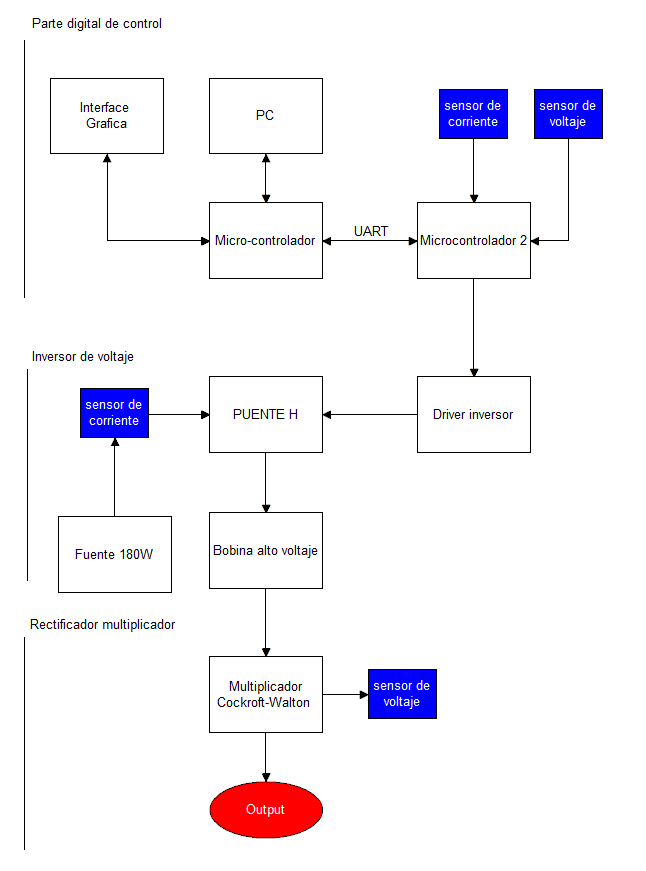
\includegraphics[width=12cm]{capitulo2/figs/figura1.png}
\caption{Calculo de ancho de pistas 1}
\end{figure}

\begin{figure}[H]
\centering
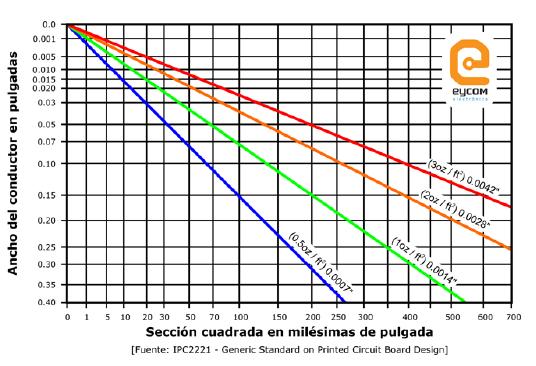
\includegraphics[width=12cm]{capitulo2/figs/figura2.png}
\caption{Calculo de ancho de pistas 1}
\end{figure}

\newpage
\section{Fuente de voltaje lineal}
Es común en proyectos de electrónica no especializados la utilización de diferentes tipos de fuentes de voltaje, entre las que se encuentran fuentes lineales, conmutadas, boost o tipo buck y los problemas que puede causar la falta de atención en este punto tan crucial puede afectan los resultados finales de un proyecto. Es por ello que se necesita conocer los principios fundamentales que reinan a este tipo de sistemas que gobernaran el comportamiento de nuestro proyecto al nivel mas básico.\\

La fuente de voltaje lineal consiste en un sistema sencillo y estructurado, el cual se diseña en diferentes configuraciones en cada modulo a partir del tipo de carga que requiere el proyecto. Para ello podemos observar en la figura 2.5 de manera ilustrativa el orden de la estructura básica de una fuente lineal.

\begin{figure}[H]
 \centering
 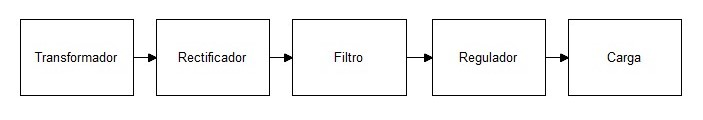
\includegraphics[width=12cm]{capitulo2/figs/fuentelineal.jpg}
 \caption{estructura fuente lineal}
 \end{figure}
 
 De manera independiente podemos analizar cada aspecto presentado en la imagen, el cual, de uno en uno se va realizando un análisis para definir los valores y topologias que satisfacen las necesidades requeridas. Tomando en cuenta lo mencionado podemos comenzar a definir las ecuaciones y modelos existentes.

\subsection{Etapa de transformador monofasico}

Esta etapa consta básicamente de un transformador que esta formado por un bobinado primario y uno o varios bobinados secundario, que tiene como función principal
convertir la energía eléctrica alterna de la red, en energía alterna de otro nivel de voltaje, por medio de la acción de un campo magnético. Ademas provee una aislación galvánica entre la entrada y la salida.\\

Los transformadores son máquinas estáticas con dos devanados, de corriente alterna enrollados sobre un núcleo magnético. El devanado por donde entra energía al transformador se denomina primario y el devanado por donde sale energía hacia las cargas que son alimentadas por el transformador se denomina secundario. El devanado primario tiene $N_{1}$ espiras y el secundario tiene $N_{2}$ espiras. El circuito magnético de esta máquina lo constituye un núcleo magnético sin entrehierros, el cual no está realizado con hierro macizo sino con chapas de acero al silicio apiladas y aisladas entre sí. De esta manera se reducen las pérdidas magnéticas del transformador.\\

Al inducir una corriente sobre cualquiera de los dos devanados se genera un flujo alterno en el núcleo magnético. Este flujo magnético se describe mediante la Ley de Faraday y produce una fuerza electromotriz que da lugar a una tensión $V_{2}$ en los bornes de dicho devanado.\\

Normalmente, para un transformador reductor o un transformador elevador tienen dos devanados que se denominan de alta tension y de baja tensión, siendo bobina primaria y bobina secundaria respectivamente. El transformador es una maquina reversible. Un mismo transformador puede alimentarse por el lado A.T. y funcionar como transformador reductor o alimentarse por el lado de B.T. y actuar como un transformador elevador.

\begin{figure}[H]
\centering
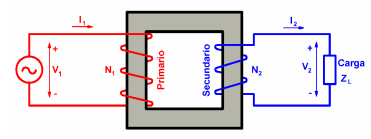
\includegraphics[width=9cm]{capitulo3/figs/trans.png}
\caption{ Principio de funcionamiento de un transformador monofásico.}
\end{figure}

En la figura 2.5 podemos observar los símbolos mas comunes que representan al transformador. 

\begin{figure}[H]
\centering
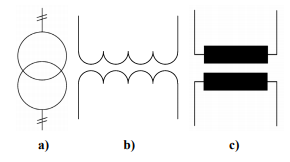
\includegraphics[width=7cm]{capitulo3/figs/simbolos.png}
\caption{ Simbologia de un transformador monofásico.}
\end{figure}

Ahora podemos definir los valores asignados o nominales para el diseño de un transformador.\\

Las \textbf{tensiones asignadas o nominales} ($V_{1}$, $V_{2}$) son aquellas para las que se ha diseñado el transformador, estas tenciones son proporcionales al numero de espiras ($N_{1}$,$N_{2}$) de cada devanado.\\

La \textbf{potencia asignada o nominal} ($S_{N}$) la cual permite un funcionamiento sin calentamientos peligrosos en su funcionamiento normal. Cabe mencionar que los dos devanados siempre tendrán la misma potencia asignada.\\

Las \textbf{corrientes nominales o asignadas} ($I_{1N}$,$I_{2N}$) se obtienen a partir de las tensiones asignadas y de la potencia asignada. Así, en un transformador monofásico se tiene que:

\begin{equation}\label{eq:ej}
S_{N}=V_{1N}*I_{1N}=V_{2N}*I_{2N}
\end{equation}
La \textbf{relación de transformación} (m) es el cociente entre las tensiones asignadas del primario y del secundario: 

\begin{equation}\label{eq:ej}
m=\dfrac{V_{1N}}{V_{2N}}
\end{equation}

Estudiando superficialmente los aspectos de construcción de un transformador, mediante estas ecuaciones podemos comenzar con la construcción y diseño. Debemos de considerar las potencias necesarias para nuestro proyecto y mediante ellas calcular el ancho del cobre y el tamaño del entre-hierro.\cite{transformador}

\subsection{Rectificador monofasico de onda completa}

El circuito rectificador de onda completa enera una señal de corriente directa (D.C.) a partir de una señal de corriente alterna
(A.C.) con todos los semiciclos de la señal, invirtiendo todos los semiciclos de una misma polaridad, para convertirlos a la otra. 

\begin{figure}[H]
\centering
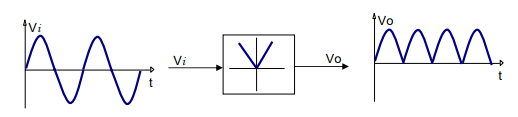
\includegraphics[width=12cm]{capitulo3/figs/puente.png}
\caption{ Simbologia de un transformador monofásico.}
\end{figure}

Para calcular el voltaje de D.C. que obtendremos podemos utilizar la siguiente ecuación\cite{rectificador}


\begin{equation}\label{eq:ej}
V_{cd}=2*0.636V_{m}
\end{equation}


\subsection{Filtros}
El voltaje de CA por lo general se conecta a un transformador, el cual lo reduce al nivel de salida de DC deseado. Un rectificador de diodos proporciona entonces un voltaje rectificado de onda completa, el cual en principio se pasa por un filtro de capacitor sencillo para producir un voltaje de DC. El cual en todos los casos presenta un voltaje de riso o variación de voltaje de CA.\\

Para calcular el voltaje de riso podemos utilizar un multimetro con capacidad de medir voltaje en CA (TRUE RMS) y el voltaje de DC. El voltimetro de cd leerá solo el nivel promedio. El medidor de ca (RMS) leerá solo el valor RMS del componente de ca del voltaje de salida. Entonces, definimos el riso como:\\

\begin{equation}
r=\frac{voltaje\:  de\:  riso\:  (rms)}{voltaje\:  de\:  DC}=V_{cd}\cdot 100\%
\end{equation}

\begin{figure}[H]
\centering
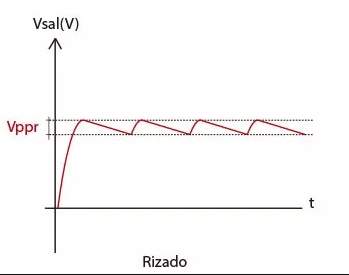
\includegraphics[width=7cm]{capitulo3/figs/risado.png}
\caption{ Forma de onda de un voltaje filtrado que muestra voltajes de dc y de rizo.}
\end{figure}

\begin{figure}[H]
\centering
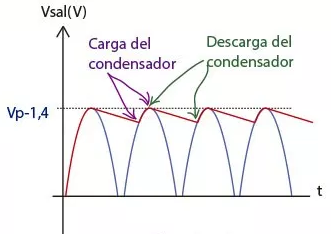
\includegraphics[width=7cm]{capitulo3/figs/filtro.png}
\caption{ Forma de onda de un voltaje filtrado que muestra voltajes de dc y de rizo.}
\end{figure}

Para nuestro caso utilizaremos un filtro de capacitor. Se conecta un capacitor en la salida del rectificador y se obtiene un voltaje de dc a través del capacitor como se muestra en la figura 2.7 y 2.8. Podemos calcular el \textbf{voltaje del riso} que obtendremos mediante la ecuación:

\begin{equation}
V_{r}(rms)=\dfrac{I_{cd}}{4\sqrt{3}fC}=\dfrac{2.4V_{cd}}{R_{L}C}
\end{equation}

Con la ecuación 2.4 podemos intuir y definir la expresion para el \textbf{rizo} de la forma de onda de salida de un rectificador de onda completa y el circuito de capacitor de filtrado:

\begin{equation}
r=\dfrac{V_{r}I_{cd}}{CV_{cd}}*100\%=\dfrac{2.4}{R_{L}C}
\end{equation}
\subsection{Regulador}

Un factor de importancia en una fuente de alimentación es la cantidad de cambios de voltaje de salida de cd a lo largo de la operación de un circuito. El voltaje provisto al a salida en la condición sin carga (sin que demande corriente de la fuente) se reduce cuando se extrae corriente de carga de la fuente. La cantidad que el voltaje de dc cambia entre las condiciones sin carga y con carga la describe un factor llamado regulación de voltaje, para una fuente ideal la regulación de voltaje seria del 0\%. Entonces podemos definir la regulacion de voltaje como:


$$regulación de voltaje = \dfrac{Voltaje sin carga - Voltaje con carga}{voltaje con carga}$$
\begin{equation} 
 \%V.R. = \dfrac{V_{NL}-V_{FL}}{V_{FL}}*100\%
\end{equation}





\newpage

\section{Inversores de voltaje}

\section{Fuentes de alto voltaje mas comunes}


\section{Multiplicador de voltaje Cockcroft-Walton}
fgdgf